\newpage

\section{Theoretical Analysis}
\label{sec:analysis}

\subsection{Operating Point}

When it comes to operating point analysis, the capacitors behave as open circuits, for their impedance is infinite, therefore, for the gain stage we can compute the Thévenin's equivalent of the bias circuit, making it easier to analyse. Running simple mesh analysis, and knowing the NPN transistor works in FAR, we can calculate every current and voltage.
To compute the input and output impedance regarding this stage and its gain, one has to analyse the incremental circuit for medium frequencies, the ones that belong to the passband, using the calculations shown in the class slides. The table below shows all these results.

\begin{center}
\begin{tabular}{|l|r|}
  \hline    
  {\bf Variable} & {\bf Value} \\ \hline
  \input{../mat/gainteo.tex}
\end{tabular}
\end{center}

For the output stage we do the same analysis but with the supermesh and this time the transistor is PNP. We calculate essentially the same variables:

\begin{center}
\begin{tabular}{|l|r|}
  \hline    
  {\bf Variable} & {\bf Value} \\ \hline
  \input{../mat/outputteo.tex}
\end{tabular}
\end{center}


Combining both stages, we get the total gain, imput and output impedances:

\begin{center}
\begin{tabular}{|l|r|}
  \hline    
  {\bf Variable} & {\bf Value} \\ \hline
  \input{../mat/totalteo.tex}
\end{tabular}
\end{center}

\newpage

\subsection{Incremental analysis}

This time, we create our incremental circuit that combines both stages as shown in figure \ref{fig:circuit-inc}.


\begin{figure}[H] \centering
\includegraphics[width=0.65\linewidth]{circuit-inc.pdf}
\caption{Incremental analysis circuit}
\label{fig:circuit-inc}
\end{figure}

Performing nodal analysis for frequency $\in [1Hz, 100MHz]$, with 10 points per decade, we get a vector with the several gain values, which we plot in a dB graph.

\begin{figure}[H] \centering
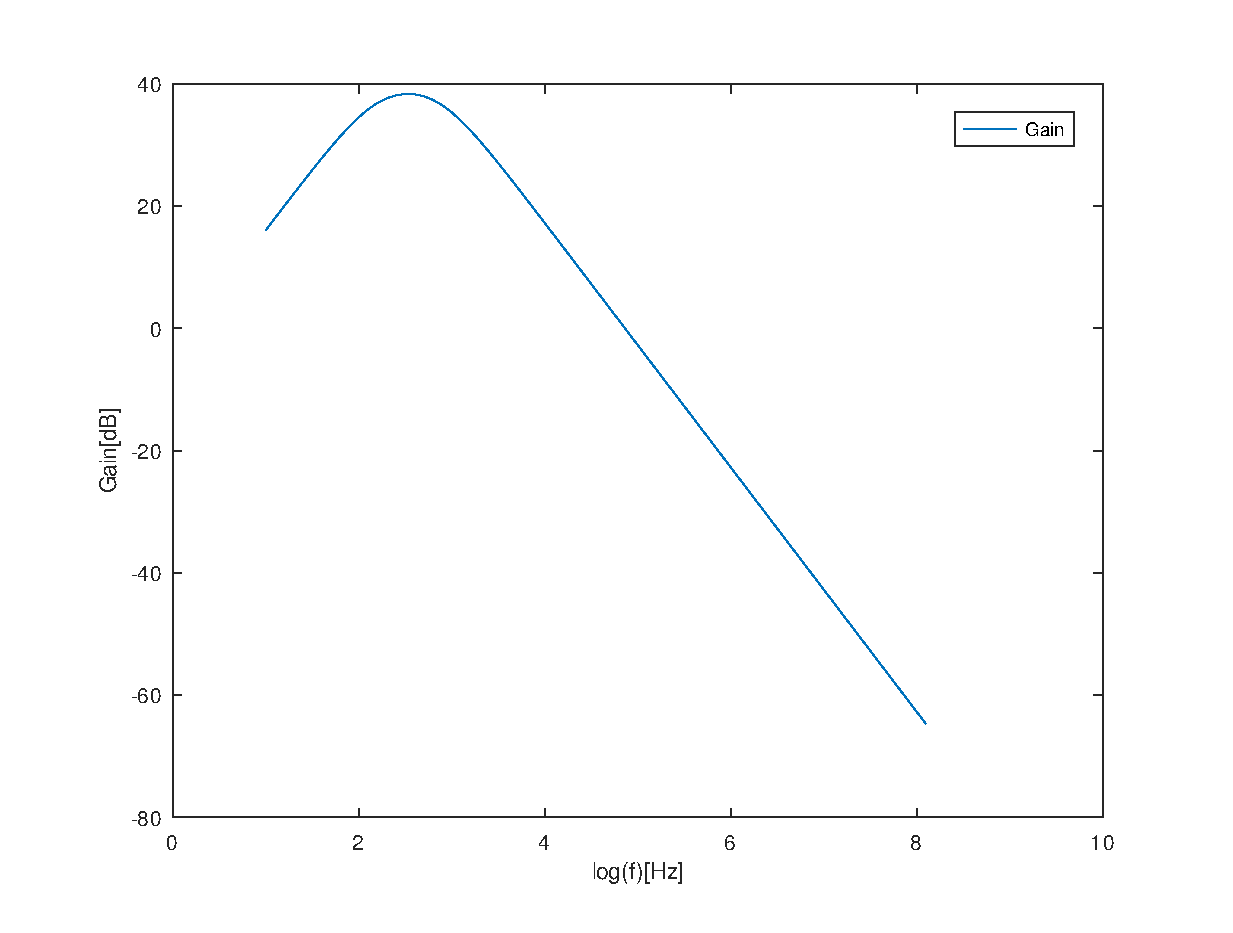
\includegraphics[width=0.5\linewidth]{gainteo.eps}
\caption{Gain in dB}
\label{fig:grafteo}
\end{figure}